% Created 2017-11-12 Sun 14:11
\documentclass{article}
\usepackage[utf8]{inputenc}
\usepackage[T1]{fontenc}
\usepackage{fixltx2e}
\usepackage{graphicx}
\usepackage{longtable}
\usepackage{float}
\usepackage{wrapfig}
\usepackage{rotating}
\usepackage[normalem]{ulem}
\usepackage{amsmath}
\usepackage{textcomp}
\usepackage{marvosym}
\usepackage{wasysym}
\usepackage{amssymb}
\usepackage{hyperref}
\tolerance=1000
\usepackage{tabularx,graphicx,ragged2e,booktabs,caption,float}
\usepackage[margin=0.8in]{geometry}
\usepackage{amsmath}
\usepackage{gensymb}
\usepackage{authblk}
\setlength{\parskip}{0.2cm}
\setlength{\parindent}{0.85cm}
\author{Tiankai Xiong}
\date{\today}
\title{PC5215, Lab3}
\hypersetup{
  pdfkeywords={},
  pdfsubject={},
  pdfcreator={Emacs 25.3.1 (Org mode 8.2.10)}}
\begin{document}

\maketitle

\section{Introduction}
\label{sec-1}

In this report, we demonstrate the study of specific heat capacity
and average spin of a graphene-like two dimensional lattice using
Ising model. Here we assume that there is no external magnetic
field. Hence the simplified Hamiltonian of the lattice is:

$$H(\sigma) = - \sum_{\langle i, j\rangle}J_{ij} \sigma_i \sigma_j$$

We calculate the specific heat capacity with formula:

$$c = \frac{1}{k_B T^2 N}(\langle E^2 \rangle - \langle E \rangle ^2)$$

The average spin will be simply:

$$s = |\frac{1}{N} \sum_i^N \sigma_i|$$

\section{Method}
\label{sec-2}

\subsection{Construction of lattice}
\label{sec-2-1}

The difference of a honeycomb lattice from a square lattice is that
not all sites are equivalent. Consequently, we should not simply
connect two sites at boundaries to create a continuous
lattice. Fortunately, we can utilize the concept of unit cell. To
illustrate, refer to Figure \ref{fig:graphene}. To construct this
two dimensional lattice, three indices are required: i and j
respectively for row and column number of the unit cell, $k\in [0,
   2)$ to index the site within its unit cell. We have to thus create
a three dimensional array in c. This isn't difficult as it is
simply an extension of the construction of two dimensional arrays.

\begin{figure}[H]
  \centering
  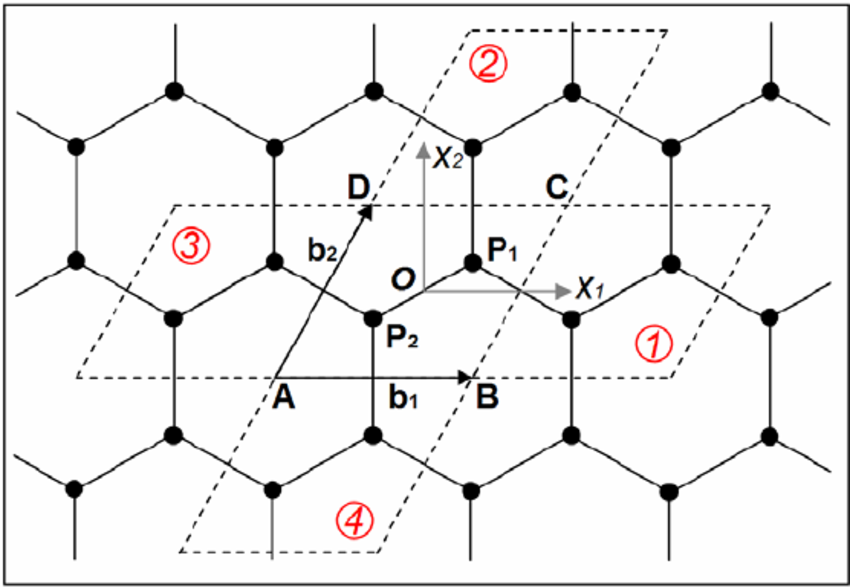
\includegraphics[width = 0.7\textwidth]{figures/graphene.jpg}

  \caption{Unit cells of a honeycomb lattice. (e.g. ABCD) While individual sites are not equivalent, all unit cells are equivalent. When we calculate spin interaction, we consider b_2 - P_2, b_1 - P_2, P_1 - P_2 \; for \; P_2 \; and \; X_1 - P_1, X_2 - P_1, P_2 - P_1 \; for \; P_2.}
  \label{fig:graphene}
\end{figure}

Another concern is the initiation of lattice. Two candidate methods exists:

\begin{enumerate}
\item Initiate each site with random spin. i.e. -1 or +1
\item Initiate all sites with identical spin.
\end{enumerate}

The first method will initiate a lattice at infinite temperature
while the second will initiate a lattice at absolute zero
temperature. When we iterate over such lattices at higher
temperature, both two lattices will approach their equilibrium
state after few sweeps. However, the difference is significant at
low temperature. For the second method, since the lattice is
initiated at zero absolute temperature, it is already at
equilibrium state and we face no problem. On the contrary, if we
initiate it with infinite temperature, it would be very hard for
the lattice to reach the equilibrium state at absolute zero
temperature. The reason is that, at very low temperature, the sites
are flipped solely depending on whether it will produce lower
energy. That is to say, it is solely decided by the random choice
while the other degree of randomness introduced by Metropolis
algorithm does not contribute significantly. Therefore, it would
take much more computational time to reach equilibrium state at
lower temperature. With the second method's advantage, we choose to
initiate the lattice with identical sites.

\subsection{One sweep over the lattice}
\label{sec-2-2}

We want to randomly select a site on the lattice. This can be
achieved by picking a random integer of $i \in [0, N)$, $j \in [0,
   N)$ and $k \in [0, 2)$. To carry out Monte Carlo, Instead of
calculating the energies before and after the flip, we simply
calculate the energy difference brought by such flip. Because each
site is connected to three other sites, and flipping one site only
affects its immediate neighbors, we only have to calculate the
energies before and after the flip in that particular
neighborhood. (i.e. three site-site interactions) The probability
of any configuration is

$$P(\sigma) = \frac{e^{-\beta H(\sigma)}}{Z}$$

where $Z$ is the normalization constant

$$Z = \sum_{\sigma} e^{-\beta H(\sigma)}$$

and $\beta$ is the inverse temperature

$$\beta = \frac{1}{k_B T}$$

Calculating the normalization constant would consume much
computational resources. Since what we really need is the ratio of
probability before and after the flip

$$\frac{P_2}{P_1} = e^{-\beta (H_2 - H_1)} = e^{-\beta \Delta H}$$

where the normalization constant is canceled in the division. The
only parameter we need to calculate the ratio of probability is
$\Delta H$ which is the change in energy by such flip.

Each time we choose a random site, we calculate the change in
energy hence the ratio of probability. If the ratio is greater than
1, we flip the site and continue. Otherwise, we check it against a
random value between 0 and 1 and continue if it is greater than the
random value. After $N \times N \times 2$ attempts of flip, we
complete a sweep as each site is visited once on average. At the
end of each sweep, we calculate the total energy and the average spin.

\subsection{Sweep for many times}
\label{sec-2-3}

We need to sweep the lattice for a large number of times so that we
collect enough data to calculate average values of energy (for heat
capacity) and average spin. The first 10\% of sweeps are discarded
because the lattice has not approached the equilibrium state. Only
the rest of data are collected. At each temperature, one of such
calculated specific heat capacity and average spin is considered
one data point.


\subsection{Multiple data points at each temperature}
\label{sec-2-4}

The above process is repeated at each temperature for at least 30
times so that the sample has statistical significance. In order to
make each data point independent of each other, we re-initiate the
lattice before each iteration. We calculate the corrected sample
error from data by:

$$s = \sqrt{\frac{1}{N(N -1) } \sum_i^N (x_i - \bar{x})^2}$$

At each temperature, for both specific heat capacity and average
spin, we have a data point

$$(\text{Temperature}\quad \text{mean value} \quad \text{corrected sample error})$$

which allows us to plot the specific heat capacity/average spin
against dimensionless temperature with error bars.

\subsection{Calculating for a range of temperature}
\label{sec-2-5}

We iterate with step = 0.1 from 0.1 to 5 dimensionless temperature.

\section{Results}
\label{sec-3}

The plot of specific heat capacity and average spin against
dimensionless temperature is presented in Figure
\ref{fig:10_30_100}, \ref{fig:20_30_100}, \ref{fig:10_100_100},
\ref{fig:10_30_1000} and \ref{fig:100_30_100}. The dimensionless
critical temperature $T_c$ is at around 1.5 units. For square
lattice, this value is at about 2 units. This shows that phase
transition of honeycomb lattice happens at a lower temperature than
square lattice.

\begin{figure}[H]
  \centering
  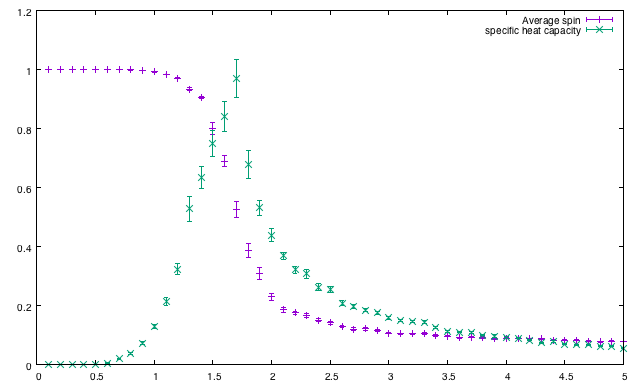
\includegraphics[width = 0.7\textwidth]{figures/200_sites_100_iterations_30_samples.png}
  \caption{200 sites, 30 samples, 100 iterations per data point}
  \label{fig:10_30_100}
\end{figure}

\begin{figure}[H]
  \centering
  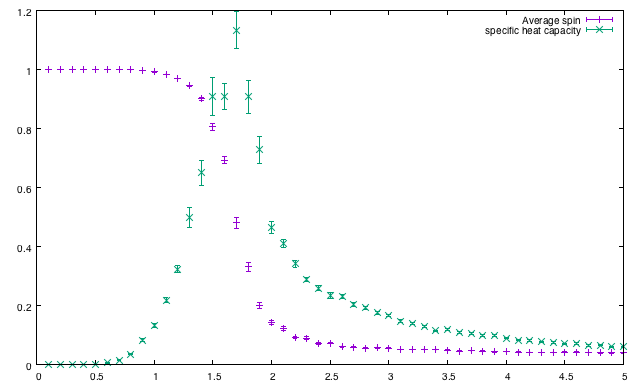
\includegraphics[width = 0.7\textwidth]{figures/800_sites_100_iterations_30_samples.png}
  \caption{800 sites, 30 samples, 100 iterations per data point}
  \label{fig:20_30_100}
\end{figure}

\begin{figure}[H]
  \centering
  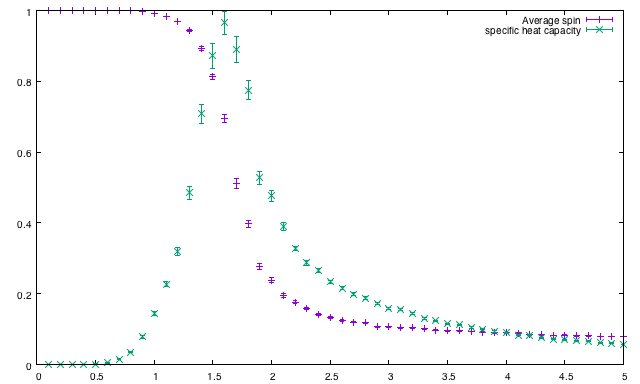
\includegraphics[width = 0.7\textwidth]{figures/200_sites_100_iterations_100_samples.png}
  \caption{200 sites, 100 samples, 100 iterations per data point}
  \label{fig:10_100_100}
\end{figure}


\begin{figure}[H]
  \centering
  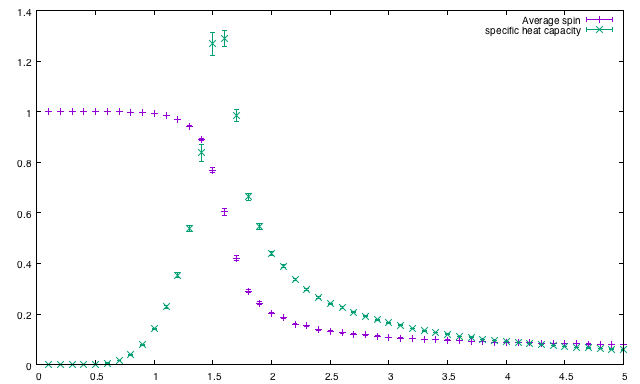
\includegraphics[width = 0.7\textwidth]{figures/200_sites_1000_iterations_30_samples.png}
  \caption{200 sites, 30 samples, 1000 iterations per data point}
  \label{fig:10_30_1000}
\end{figure}


\begin{figure}[H]
  \centering
  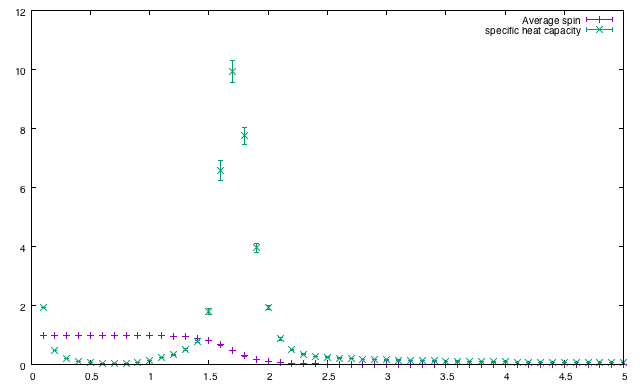
\includegraphics[width = 0.7\textwidth]{figures/20000_sites_100_iterations_30_samples.png}
  \caption{20000 sites, 30 samples, 100 iterations per data point}
  \label{fig:100_30_100}
\end{figure}

\section{Discussion}
\label{sec-4}

At lower temperature, the equilibrium state is so that the lattice
is polarized thus we have a high average spin. On the contrary, at
high temperature, the access kinetic energy allows more flips thus
renders the lattice non-polar. The transition between polar and
non-polar occurs at the critical temperature $T_c$.

As for specific heat capacity, which depends on the standard
deviation of energy of the lattice, its value would be lower when
the lattice is far from phase transition as the equilibrium state is
achieved. However, at temperature near critical temperature where
phase transition occurs, the equilibrium state is not well defined
thus the fluctuation of total energy is large, contributing to a
large specific heat capacity.

The peak of specific heat capacity and the transition of average to
spin occur at the same dimensionless temperature, $T_c$.

When we increase the lattice size, the peak of specific heat
capacity increases. This is a result of increasing total energy.

\section{SRC}
\label{sec-5}

\hline
\begin{verbatim}
#include<stdio.h>
#include<stdlib.h>
#include<math.h>

#define EPS 0.1

void create_lattice(int ***lattice, int N){
  /*
    The lattice is created by grouping two C atoms in the same unit
    cell. By doing so, we have a 2D array of unit cells, with each
    unit cell equivalent to the others. Consequently, when we want to
    join two atoms from two boundaries, it will always to atom 1
    connected to atom 2.
   */
  for(int i = 0; i< N; i++){
    lattice[i] = malloc(N * sizeof(int*));
    for(int j = 0; j<N; j++){
      lattice[i][j] = malloc(2 * sizeof(int));
      for(int k = 0; k<2; k++){
        lattice[i][j][k] = 1;
        /* This is better for the lattice at low temperature because
           it starts at equilibrium state. For high temperature, the
           kinetic energy is sufficient to alter the state to
           equilibrium */
      }
    }
  }
};

void flip_lattice(int ***lattice, int i, int j, int k){
  lattice[i][j][k] *= -1;
};

float calculate_energy(int ***lattice, int N){
  float total_energy = 0;
  for(int i = 0; i< N; i++){
    for(int j = 0; j< N; j++){
      for(int k = 0; k < 2; k++){
        if(k == 0){
          /* for the atom on the left hand side of the unit cell */
          /* its nearest neighboors are: */
          /* the other atom in the same unit cell */
          total_energy -= lattice[i][j][0] * lattice[i][j][1];
          /* the right hand side atom in the unit cell on its left */
          total_energy -= lattice[i][j][0] * lattice[i][(j-1 + N) % N][1];
          /* the right hand side atom in the unit cell below it */
          total_energy -= lattice[i][j][0] * lattice[(i-1 + N)%N][j][1];

          /* (i-1 +N)%N is used so that it joins boundaries */
        }
        else if(k == 1){
          total_energy -= lattice[i][j][1] * lattice[i][j][0];

          total_energy -= lattice[i][j][1] * lattice[i][(j+1 + N) % N][0];

          total_energy -= lattice[i][j][1] * lattice[(i+1 + N)%N][j][0];

        }else{
          printf("error!\n");
        }
      }
    }
  }
  total_energy /= 2;            /* each pair has been counted twice */
  return total_energy;
};

/* If only one site is flipped, we don't have to iterate over the
   entire lattice */
float calculate_difference(int ***lattice, int i, int j, int k, int N){
  float energy_diff = 0;
  if(k == 0){
    energy_diff += 2* lattice[i][j][0] * lattice[i][j][1];
    energy_diff += 2* lattice[i][j][0] * lattice[i][(j-1 + N) % N][1];
    energy_diff += 2* lattice[i][j][0] * lattice[(i-1 + N)%N][j][1];

  }else if(k == 1){
    energy_diff += 2* lattice[i][j][1] * lattice[i][j][0];

    energy_diff += 2* lattice[i][j][1] * lattice[i][(j+1 + N) % N][0];

    energy_diff += 2* lattice[i][j][1] * lattice[(i+1 + N)%N][j][0];

  }else{
    printf("error! k = %d\n", k);
  }

  return energy_diff;
};

void random_site(int *i, int *j, int *k, int N){
  *i = rand() % N;
  *j = rand() % N;
  *k = rand() % 2;
};




void print_lattice(int ***lattice, int N){
  for(int i =0; i< N; i++){
    printf("\n");
    for(int j = 0; j< N; j++){
      printf(" [ ");
      for(int k = 0; k< 2; k++){
        printf(" %d ", lattice[i][j][k]);
      }
      printf("] ");
    }
    printf("\n");
  }
};


float heat_capacity(float *energies, int instances, int N, float T){
  float c = 0;
  c = 1/(T*T*N*N*2);            /* remark: total number of spin is N*N*2 */
  float E_square_mean = 0, E_mean_square = 0;
  for(int i = 0; i< instances; i++){
    E_square_mean += pow(energies[i], 2);
    E_mean_square += energies[i];
  }
  E_square_mean /= instances;
  E_mean_square /= instances;
  E_mean_square = pow(E_mean_square, 2);
  c *= (E_square_mean - E_mean_square);
  return c;

};

/* the average spin of the lattice */
float average_spin(int ***lattice, int N){
  float spin = 0.0;
  for(int i = 0; i < N; i++){
    for(int j = 0; j < N; j++){
      for(int k = 0; k < 2; k++){
        spin += lattice[i][j][k];
      }
    }
  }
  spin /= (pow(N, 2) * 2);
  spin = fabs(spin);

  return spin;
};

/* the mean average spin of all iterations */
float mean_average_spin(float *spins, int instances){
  float result = 0;
  for(int i = 0; i < instances; i++){
    result += spins[i];
  }

  result /= instances;
  return result;
};

float _mean(float *sample, int instances){
  float sum = 0;
  for(int i = 0; i< instances; i++){
    sum += sample[i];
  }
  float mean = sum/(float)instances;
  return mean;
};


/* this might exist in stdlib.h, but I just redefine it here */
float corrected_sample_error(float *sample, int instances){
  float mean = _mean(sample, instances);

  float result = 0;
  for(int i = 0; i < instances; i++){
    result += pow((sample[i] - mean), 2);
  }
  return sqrt(result/(instances*(instances - 1)));
};





int main(){


  printf("What's the dimension you want to use? (total 2*N^2 sits)\n");
  char strN[10];
  scanf("%s", strN);

  printf("How many samples would you like to take?\n");
  char strSample_size[10];
  scanf("%s", strSample_size);

  printf("How many iterations would you like to run?\n");
  char strIterations[10];
  scanf("%s", strIterations);

  FILE *c_FILE;
  c_FILE = fopen("heat_capacity.dat", "w+");

  FILE *s_FILE;
  s_FILE = fopen("spin.dat", "w+");
  float total_energy;

  int N = atoi(strN);                   /* this gives us N*N*2 sites */


  int ***lattice = malloc(N * sizeof(int**));
  int i, j, k;

  int sample_size = atoi(strSample_size);
  int total_iteration = atoi(strIterations);  /* total number of sweeps */

  for(float T = 0.1; T < 5; T+=EPS){

    float *spin_record = malloc(sample_size * sizeof(float));
    /* This is to record average spin so that we can take its standard error */
    float *heat_capacity_record = malloc(sample_size * sizeof(float));
    /* The same for heat capacity */

    for(int r = 0; r < sample_size; r++){
      /* Take 30 samples such that it has statistical significance */
      create_lattice(lattice, N);


      float *energies = malloc(total_iteration * sizeof(float));
      /* an array of total energies */
      float *spins = malloc(total_iteration * sizeof(float));
      /* an array of average spings */
      int instances = 0;      /* a counter for the above two arrays */
      for(int iteration = 0; iteration < total_iteration; iteration++){
        /* Sweep over the entire lattice */
        float prob;               /* the probability of such flip */
        for(int counter = 0; counter < N*N*2; counter++){
          random_site(&i, &j, &k, N);    /* choose a random site */
          /* decide whether to accept the flip */
          /* P(configuration1)/P(configuration2) = e^{-(H2 - H1)} */
          /* k_b = 1 */
          float E_diff = calculate_difference(lattice, i, j, k, N);
          prob = exp(-E_diff/T);

          if(prob > rand()/((float)RAND_MAX+1)){

            /* if the ratio > 1, it must be bigger than the random
               value, hence we accept */
            /* else, we check it against the random float in [0, 1] */
            flip_lattice(lattice, i, j, k);
          }
        }
        /* calculate the total energy */
        total_energy = calculate_energy(lattice, N);
        if(iteration > total_iteration/10){
          energies[instances] = total_energy;
          spins[instances] = average_spin(lattice, N);
        instances++;
        }

      }
      heat_capacity_record[r] = heat_capacity(energies, instances, N, T);
      spin_record[r] = mean_average_spin(spins, instances);

    }
    fprintf(c_FILE, "%f    %f    %f\n",
            T, _mean(heat_capacity_record, sample_size),
            corrected_sample_error(heat_capacity_record, sample_size));
    fprintf(s_FILE, "%f    %f    %f\n",
            T, _mean(spin_record, sample_size),
            corrected_sample_error(spin_record, sample_size));
  }

}
\end{verbatim}

\hline
% Emacs 25.3.1 (Org mode 8.2.10)
\end{document}
